% 2010 年江苏卷第 21A 题：圆 O 的切线与直径。
% 来源 PDF：普通高考/2010/2010江苏.pdf，SHA-256 e701df878d51a700720549274fe7969bd54342f0f58acb051c516fc502b58af7。
% 原页：第 2 页（A3 三栏）第 1 栏上部，书页码 606。
% 重绘依据：AB 为直径，D 在圆上，切线 DC 交 AB 延长线于 C；DA=DC。
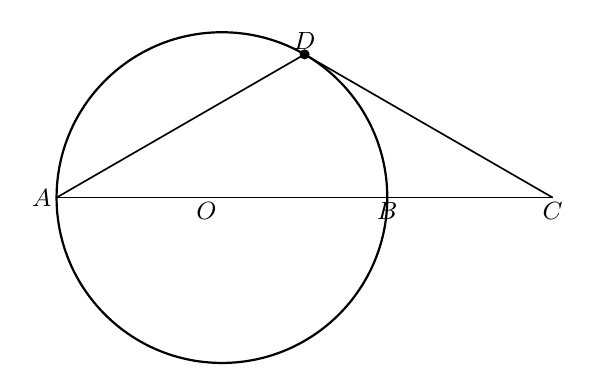
\begin{tikzpicture}[semithick, scale=1.4, every node/.style={inner sep=1.6pt, font=\small}]
  \draw[thick] (0,0) circle (1.5);
  \coordinate (O) at (0,0);
  \coordinate (A) at (-1.5,0);
  \coordinate (B) at (1.5,0);
  \coordinate (C) at (3,0);
  \coordinate (D) at (0.75,1.299);

  \draw (A) -- (C);
  \draw (D) -- (C);
  \draw (A) -- (D);
  \fill (D) circle (1.3pt);
  \node[left] at (A) {$A$};
  \node[below] at (B) {$B$};
  \node[below] at (C) {$C$};
  \node[above] at (D) {$D$};
  \node[below left] at (O) {$O$};
\end{tikzpicture}
